\documentclass[12pt,english]{article}
\usepackage[a4paper,bindingoffset=0.2in,%
            left=0.4in,right=1in,top=1in,bottom=1in,%
            footskip=.25in]{geometry}
\usepackage{amsmath}
\usepackage{graphicx}
\usepackage{float}

\graphicspath{ {./res/} }

\newcommand{\myparagraph}[1]{\paragraph{#1}\mbox{}\\}

\title{Modelare și Simulare\\Temă laborator\\-\\Tema 2\\Instalație hidraulică cu patru rezervoare}
\date{2018\\Decembrie}
\author{Ionescu Alexandru Cristian\\Pangratie Andrei\\333 AC}

\begin{document}

\maketitle

\pagebreak


\myparagraph {Introducere}
Simularea procesului este salvata cu versiunea MATLAB R2017a si pentru rularea ei se va folosi scriptul \textit{run\_tema\_2017.m}. Pentru a rula cu MATLAB R2018a se va folosi scriptul \textit{run\_tema.m}

\myparagraph {Structura proiectului}
Ficare subpunct are doua fisiere aferente (\textit{load\_workspace\_*.m} si \textit{tema\_comm\_*.m}) \\
Pentru a rula simulari individuale se pot comenta/decomenta doua cate doua liniile respective.\\
Fisierul \textit{animate\_levels.m} este folosit dupa fiecare simulare pentru a crea o reprezentare grafica a evolutiei nivelelor rezervoarelor cu apa.\\
Pentru simularile repetate, animatia se poate dezactiva prin setarea flagului: $animation\_enable = 0$

% 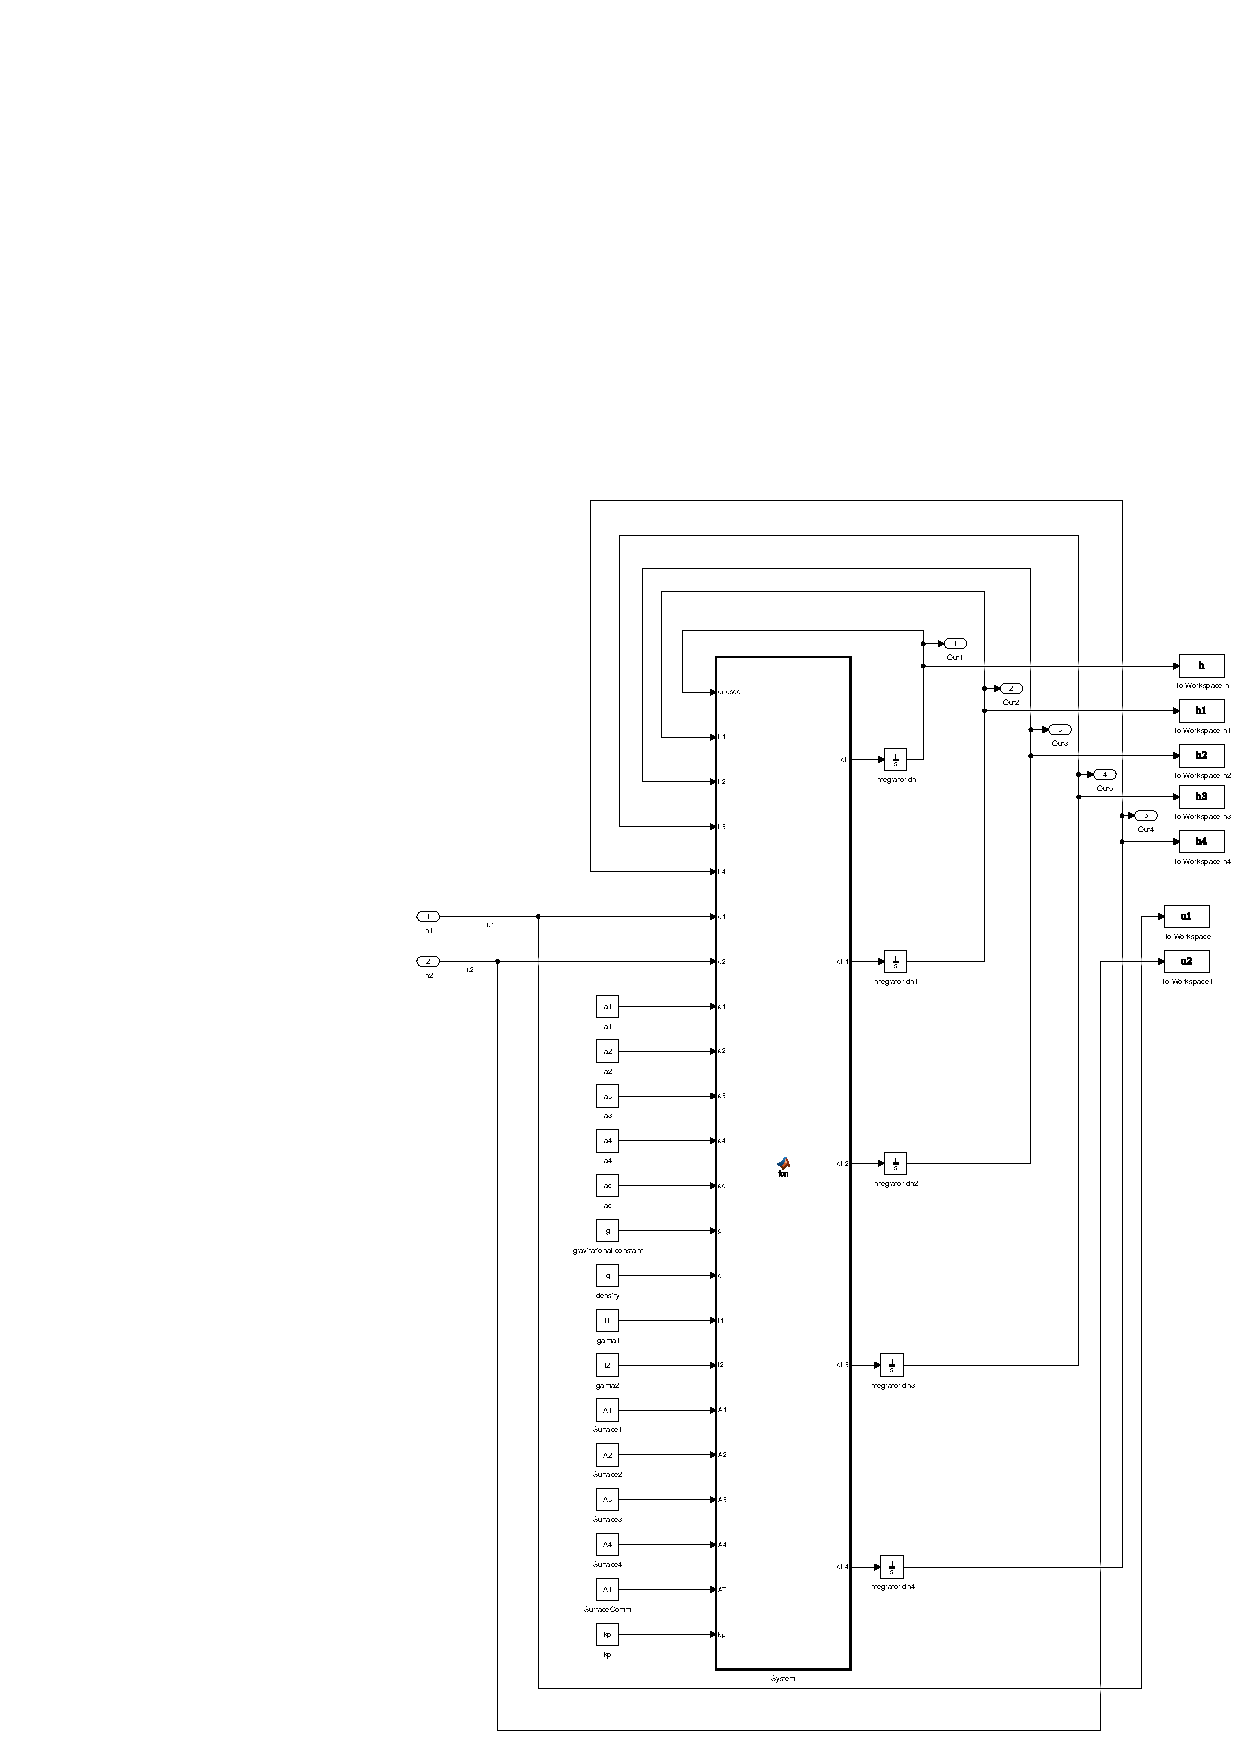
\includepdf[pages=-,pagecommand={},width=\textwidth]{system_schema.pdf}

% Consideram filtrul FIR de ordinul I:
% \begin{center}
% $\displaystyle H( z) \ =\ 1-cz^{-1} ,\ c\ =re^{j\theta } ,\ \theta \in [ 0,\ \pi ]$
% \end{center}

% \subparagraph {Pentru:\ $\displaystyle \theta \ =\ \pi /3$}

\myparagraph {Subpunctul a}

\begin{figure} [H]
	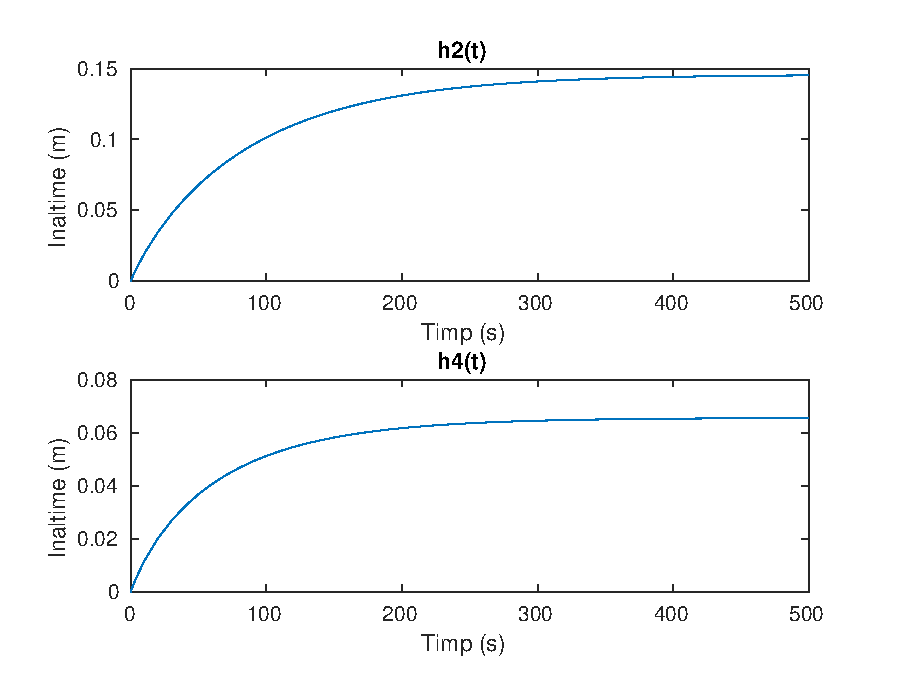
\includegraphics[width=1\textwidth]{a_2.eps}
	\caption{Evolutia iesirilor y2 si y4}
\end{figure}

\begin{figure} [H]
	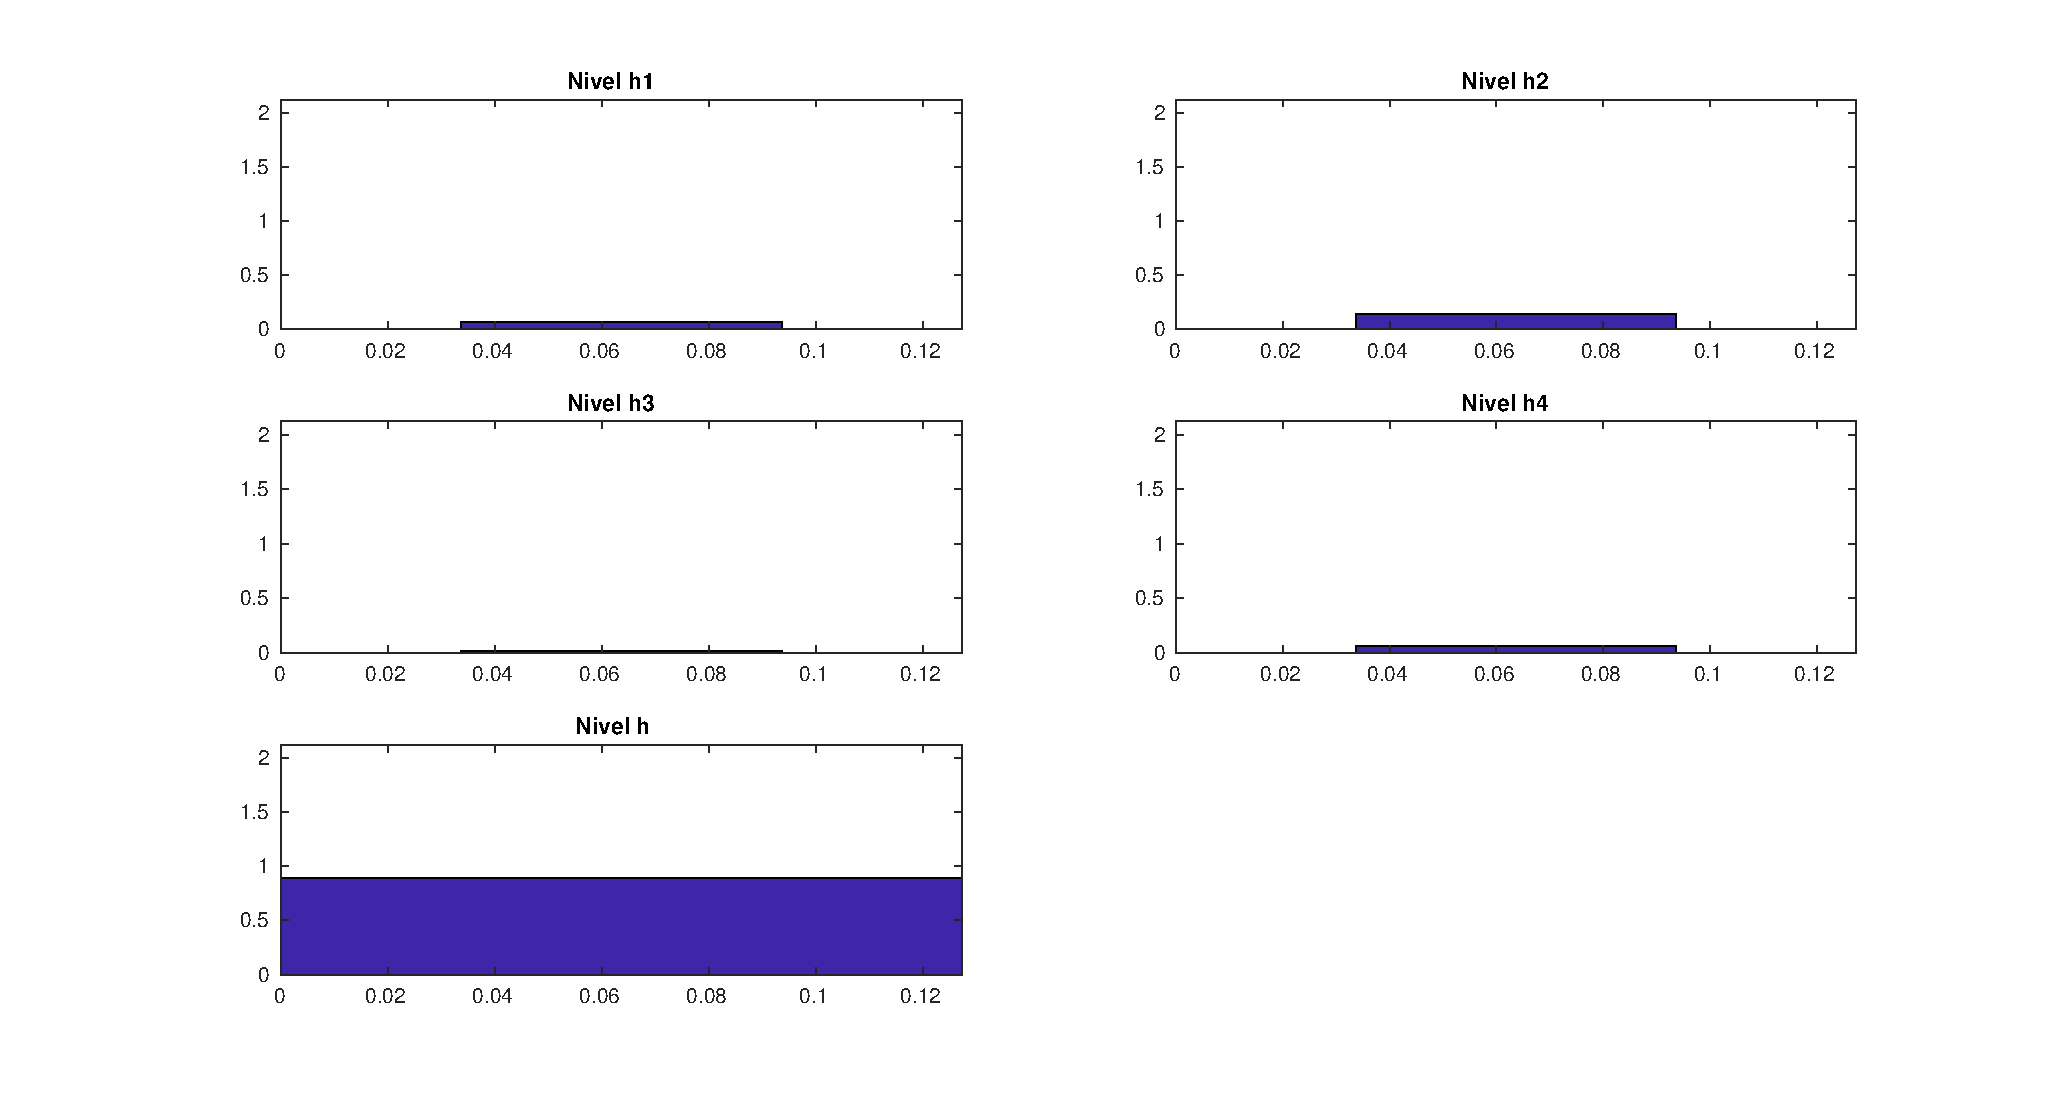
\includegraphics[width=1\textwidth]{a_1.eps}
	\caption{Exemplu animate levels}
\end{figure}

\myparagraph {Subpunctul b}
Alo

\begin{figure} [H]
	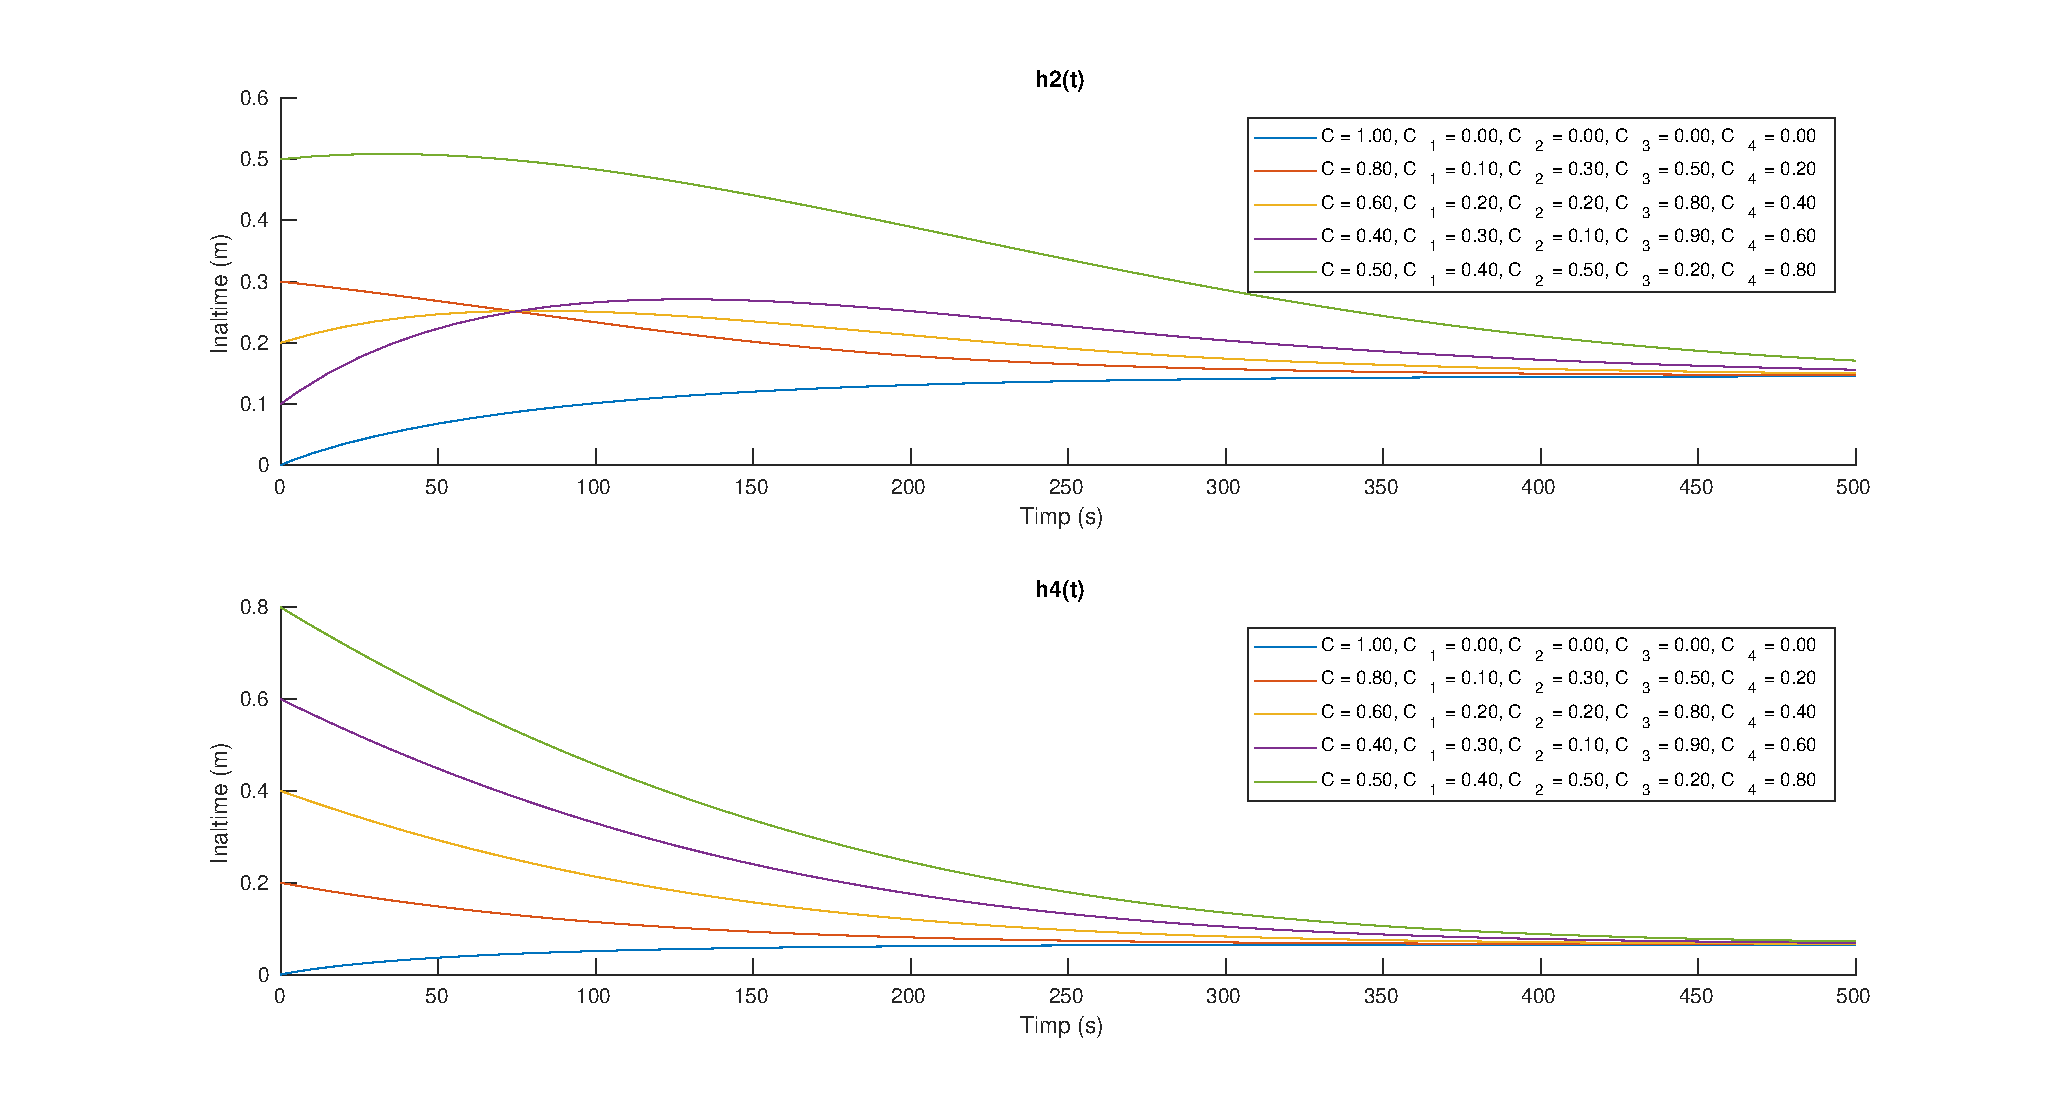
\includegraphics[width=1\textwidth]{b_1.eps}
	\caption{Evolutia iesirilor y2 si y4}
\end{figure}

\myparagraph {Subpunctul c}
Salut

\begin{figure} [H]
	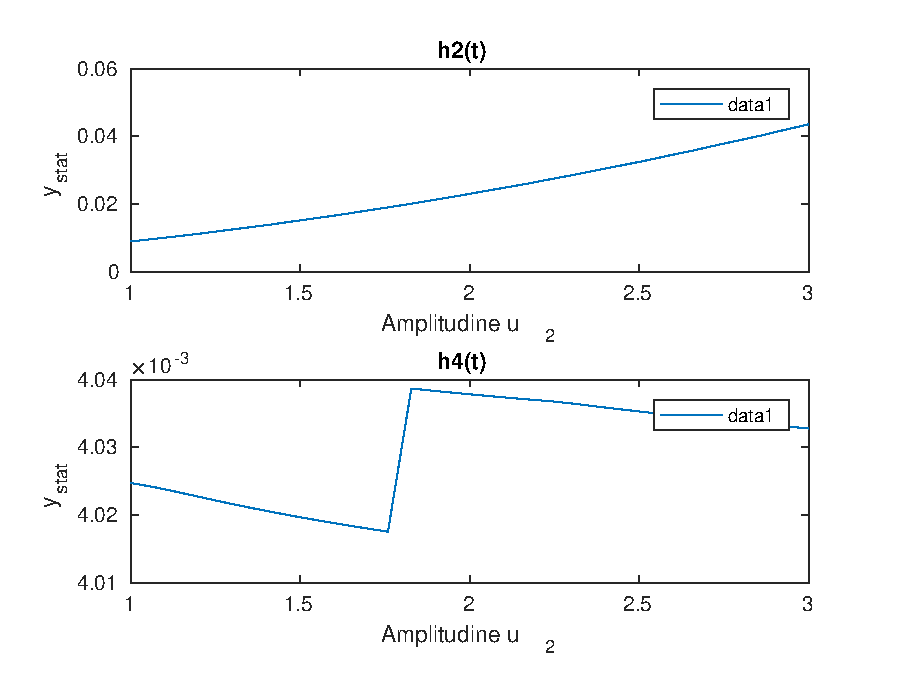
\includegraphics[width=1\textwidth]{c_1.eps}
	\caption{Evolutia iesirilor y2 si y4 in functie de valorile constantelor de integrare}
\end{figure}

\begin{figure} [H]
	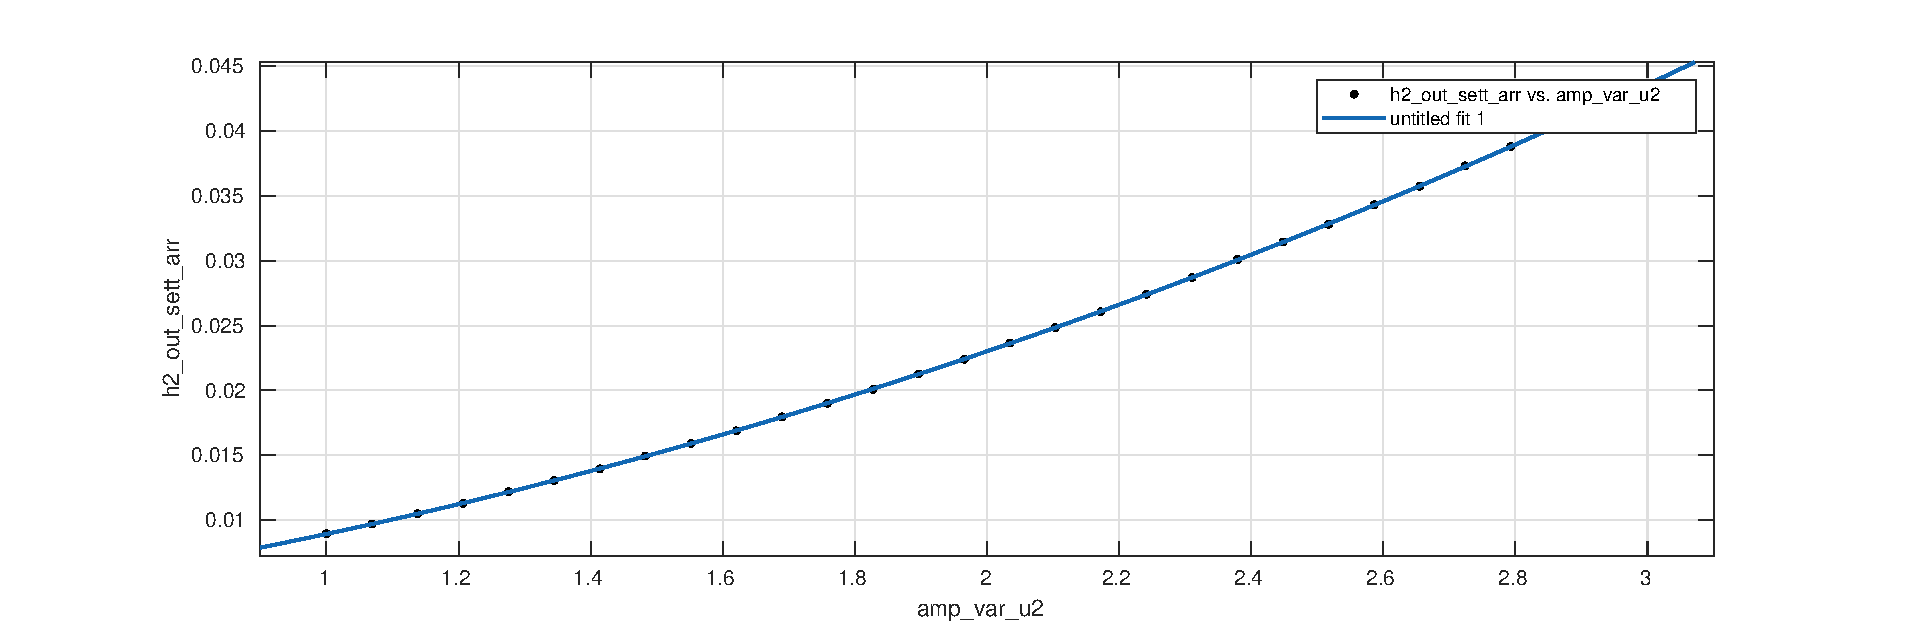
\includegraphics[width=1\textwidth]{c_2_1.eps}
	\caption{Stabilizare h2 in functie de amplitudinea intrarii}
\end{figure}

\begin{figure} [H]
	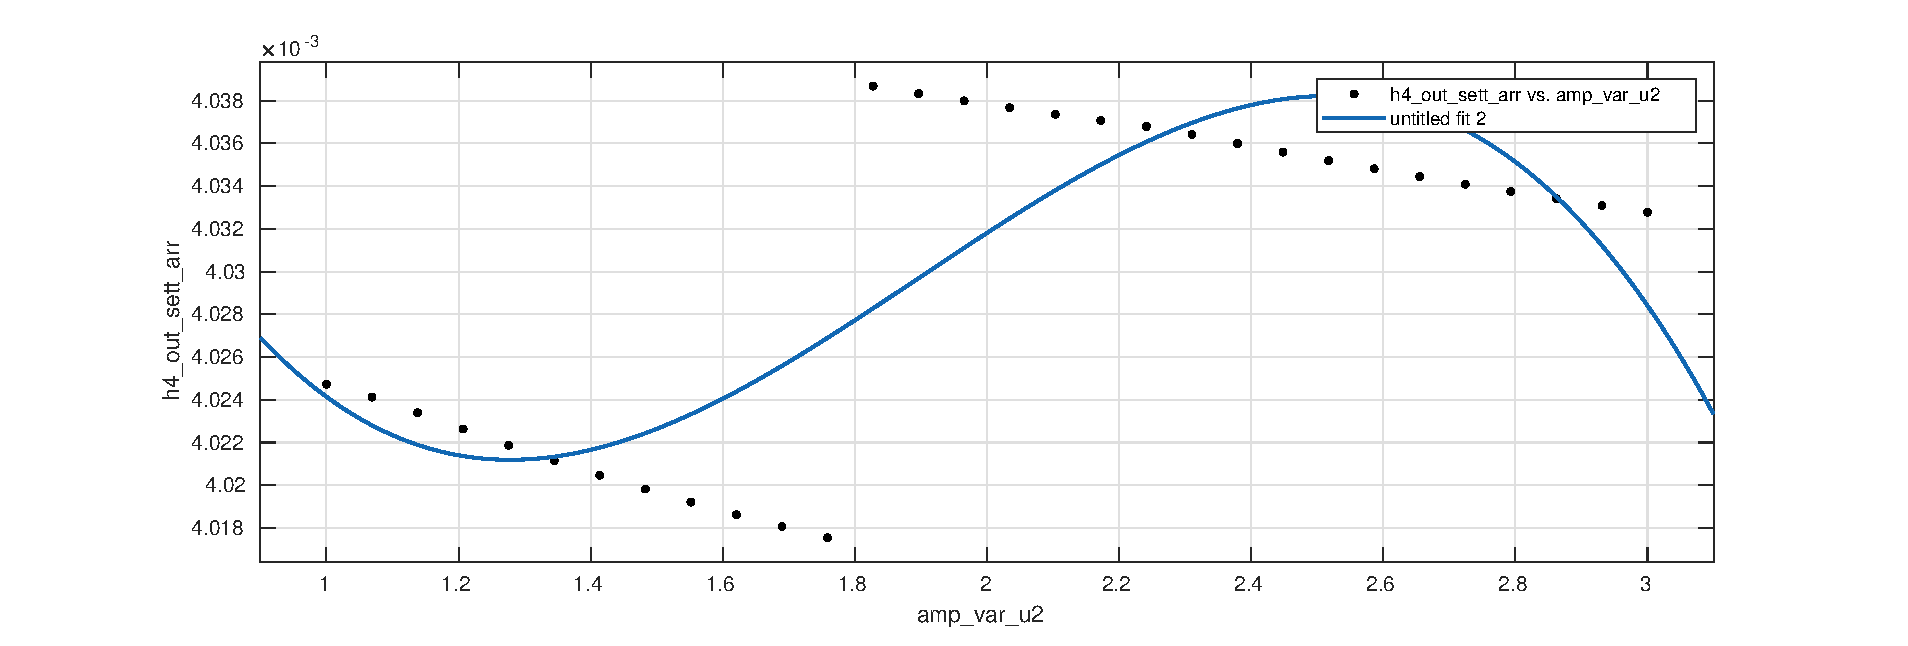
\includegraphics[width=1\textwidth]{c_2_2.eps}
	\caption{Stabilizare h4 in functie de amplitudinea intrarii}
\end{figure}

\myparagraph {Subpunctul d}

\begin{figure} [H]
	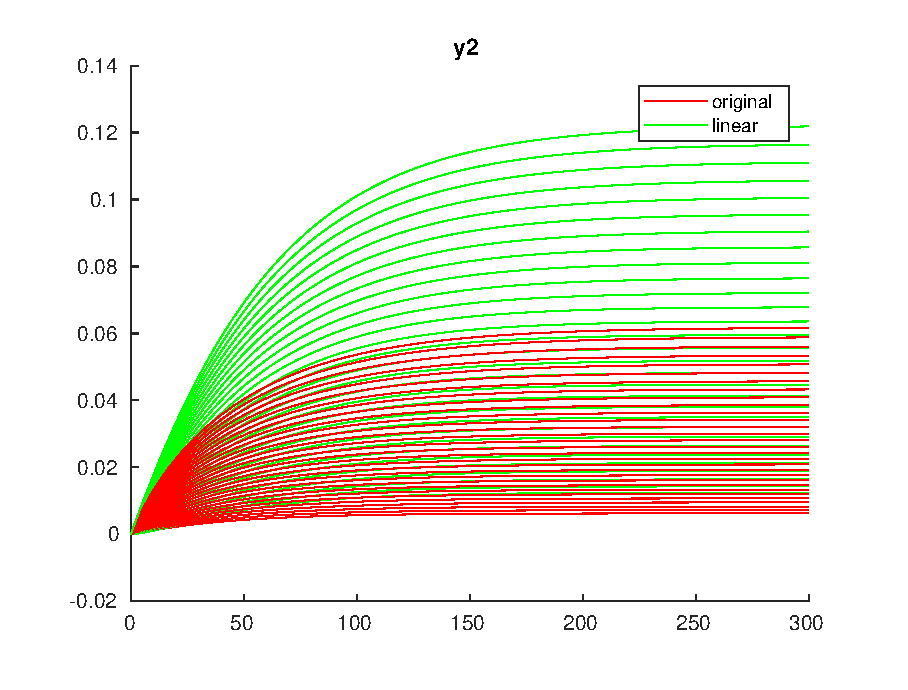
\includegraphics[width=1\textwidth]{d_1.eps}
	\caption{Evolutia iesirii h2 vs aproximarea sa liniara}
\end{figure}

\begin{figure} [H]
	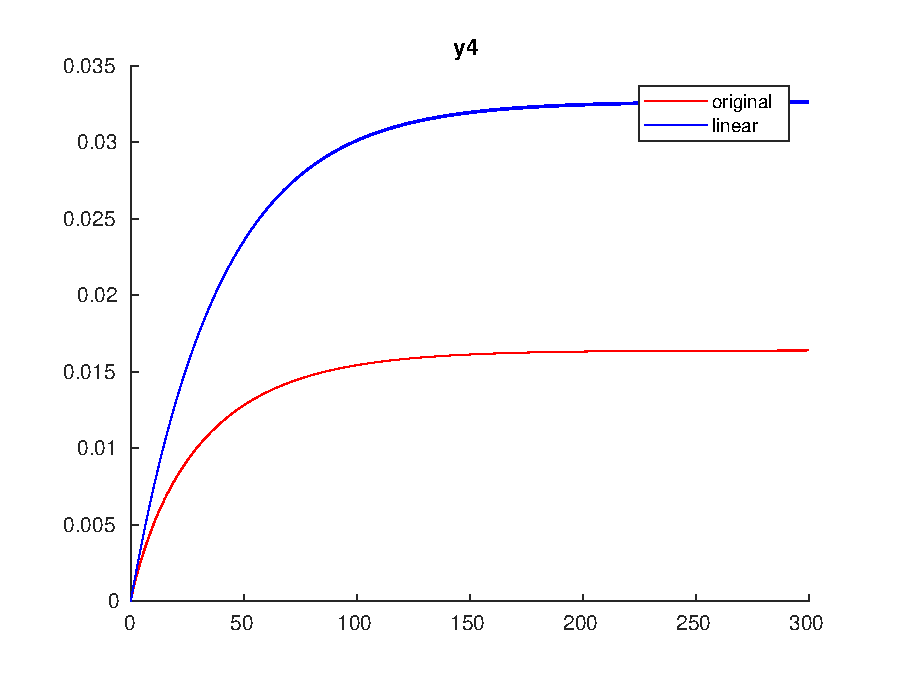
\includegraphics[width=1\textwidth]{d_2.eps}
	\caption{Evolutia iesirii h4 vs aproximarea sa liniara}
\end{figure}

\myparagraph {Subpunctul e}

\begin{figure} [H]
	\includegraphics[width=1\textwidth]{e_1.eps}
	\caption{Evolutia iesirii h2 vs aproximarea sa liniara}
\end{figure}

\myparagraph {Subpunctul f}
\myparagraph {Subpunctul g}
\myparagraph {Subpunctul h}

\begin{figure} [H]
	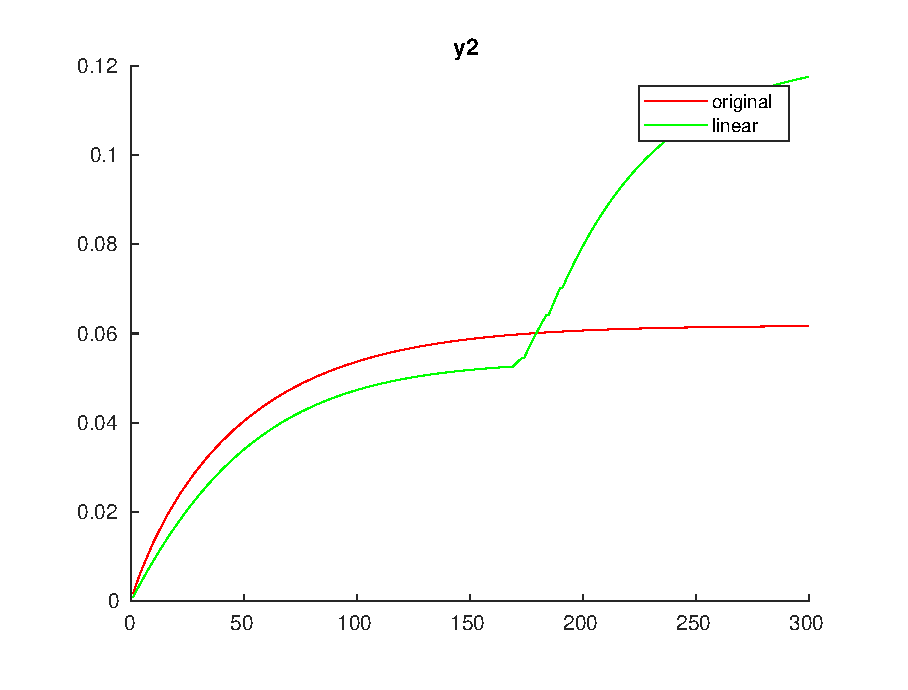
\includegraphics[width=1\textwidth]{fgh_1.eps}
	\caption{Evolutia iesirii h4 vs aproximarea sa liniara}
\end{figure}

\begin{figure} [H]
	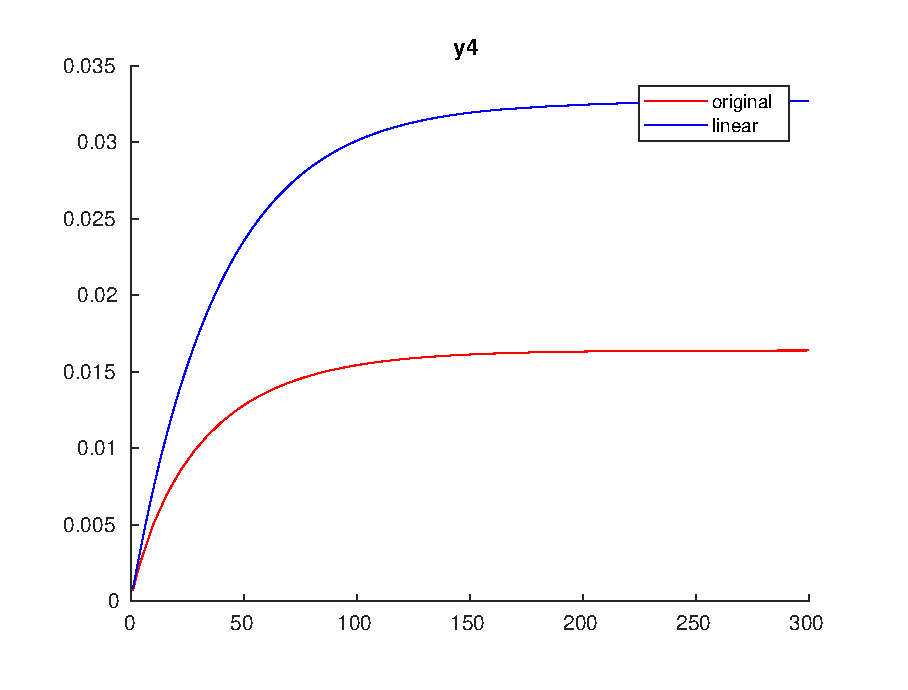
\includegraphics[width=1\textwidth]{fgh_2.eps}
	\caption{Evolutia iesirii h4 vs aproximarea sa liniara}
\end{figure}

\end{document}